%-------- Stiffness method ---------------
\section{Stiffness method}
This module allows the determination of the stiffness of an object by fitting both loading and unloading curve with a straight line. 
This method is shown unless the software was compiled without Fortran support.  \\

\begin{figure}[ht]
  \centering
  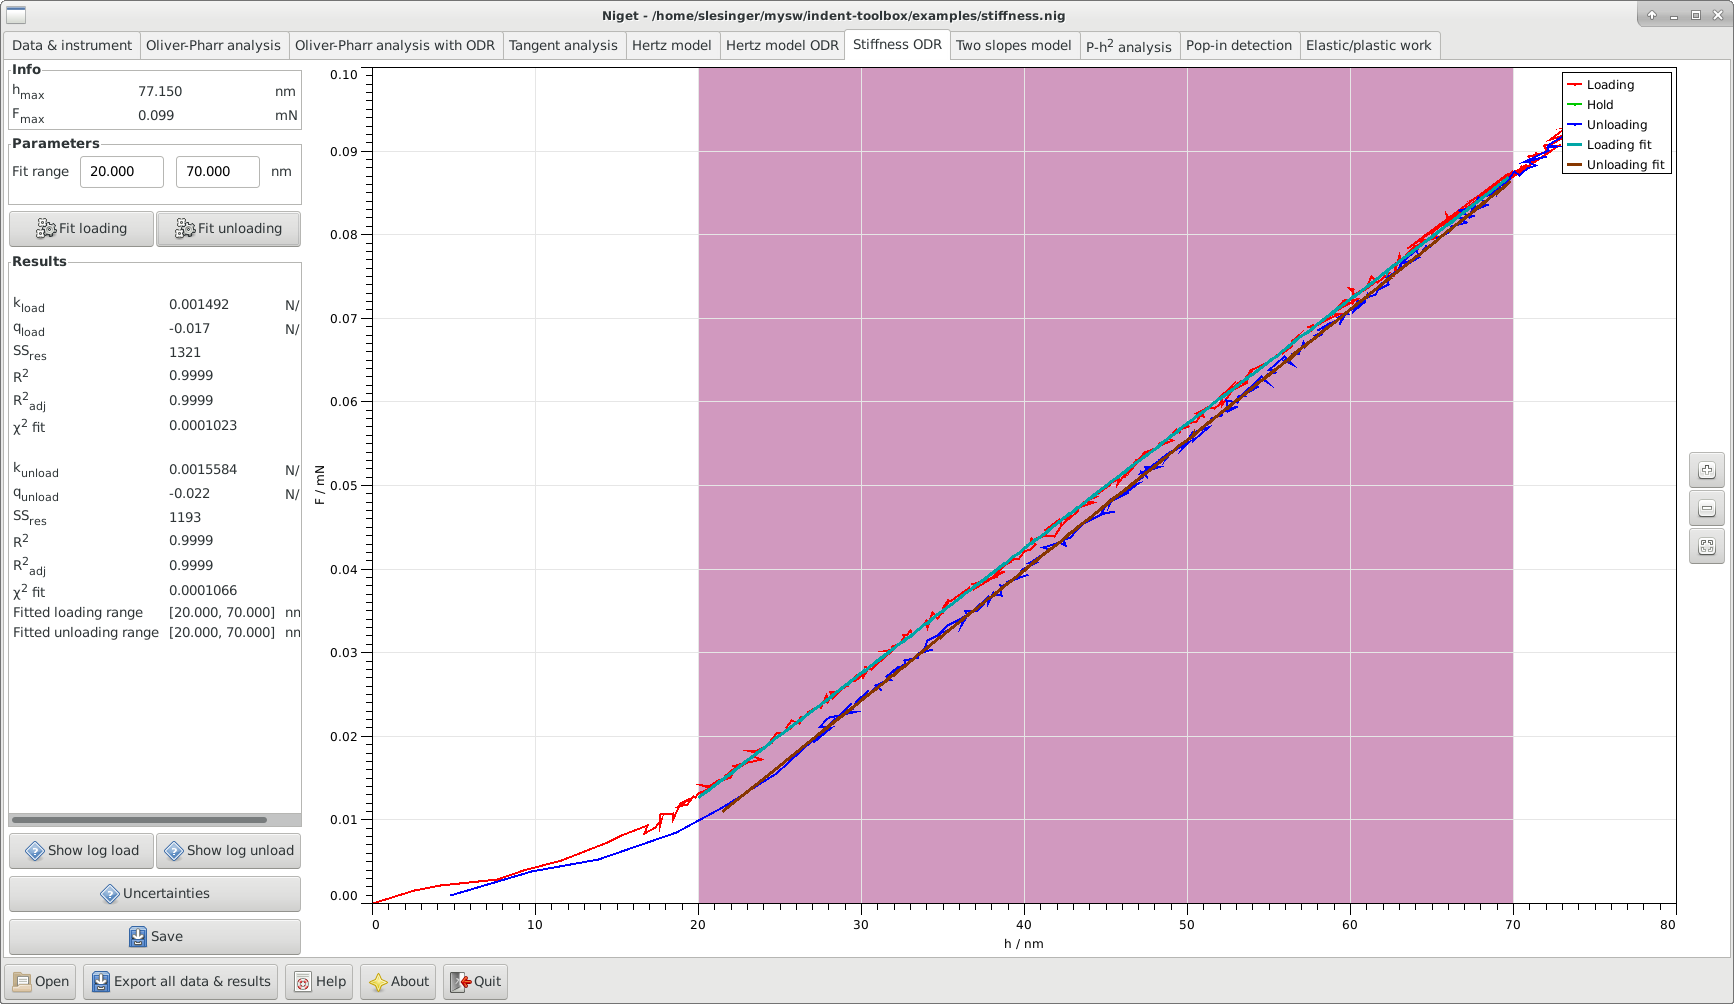
\includegraphics[width=\textwidth]{images/screen-stiffness}
  \caption{Stiffness analysis using orthogonal data regression}
\end{figure}

\subsection{Window}
The window consists of several blocks:
\begin{itemize}
 \item \emph{Info} displays the maximum depth and force during the indentation
 \item \emph{Parameters} shows the selected range in nm and in \% of the maximum force, and the correction $\beta$. 
        \begin{itemize}
          \item[-] The fitting range can be selected either using the mouse or typing in the range entries.   
        \end{itemize}
 \item \emph{Fit} buttons for indepedent fitting of the loading and unloading curves, see section \ref{stiffness_calc} for details of the calculation.
 \item \emph{Results} displays all results in the following order: 
       the slope of the loading curve $\kl$, the offset of the loading curve $\ql$, 
       the residual sum of squares of the corresponding fit and the goodness of fit parameters,
       the slope of the unloading curve $\ku$, the offset of the loading curve $\qu$,
        the residual sum of squares of the corresponding fit and the goodness of fit parameters
       and the ranges used for the fitting procedures.
       Warnings are displayed if the fittings procedures failed.
 \item \emph{Uncertainties} show the uncertainty analysis window, see section \ref{stiffness_unc}.
 \item \emph{Show log load} Show the report about the fitting procedure of the loading curve in a separate window.  The reports are saved to files \emph{fit.log.stiff.load.err} and \emph{fit.log.stiff.load.rpt}. 
 \item \emph{Show log unload} Show the report about the fitting procedure of the unloading curve in a separate window.  The reports are saved to files \emph{fit.log.stiff.unload.err} and \\ \emph{fit.log.stiff.unload.rpt}. 
 \item \emph{Save} save parameters and results to given file. 
 \item \emph{Graph} display the unloading curve and the fitted curves. Stepwise zooming/unzooming can be performed by selecting a range with the mouse and pressing the \emph{Zoom}/ \emph{Unzoom} buttons. The graph is restored to its original size by the \emph{Restore} button.
\end{itemize}

\subsection{Procedure} \label{stiffness_calc}
The stiffness analysis simply fits both loading and unloading curve with straight lines. 
\begin{enumerate} 
 \item 
 Fit the loading curve with a straight line 
$$
F = \kl h + \ql
$$
using orthogonal least squares as implemented in the package ODRPACK95 \cite{odrpack95}.
\item
Fit the unloading curve with a straight line 
$$
F = \ku h + \qu
$$
using orthogonal least squares as implemented in the package ODRPACK95 \cite{odrpack95}. 

\end{enumerate}


